\documentclass[10pt,twocolumn]{article}
\usepackage{graphicx}
\usepackage{amsmath}
\usepackage{float}
\usepackage{hyperref}
\usepackage{geometry}

% Réglages compacts
\geometry{margin=1.6cm, columnsep=1.1cm}
\setlength{\parskip}{0pt}
\setlength{\parindent}{1em}

\title{\textbf{Analyse du réseau de contacts du Malawi} \\ 
\large Application des concepts du cours et comparaison des distributions}
\author{}
\date{}

\begin{document}

\maketitle


\section{Introduction}

Ce rapport présente l’analyse détaillée du réseau de contacts en face-à-face observé 
dans un village rural du Malawi. Les données initiales proviennent de capteurs portés 
par les habitants permettant d’enregistrer des interactions de proximité à haute résolution.
Le réseau brut contenait \textbf{86 nœuds} et \textbf{347 arêtes}, dont une composante géante 
de \textbf{84 nœuds}. 

Après nettoyage (suppression des contacts nuls, agrégation des interactions et filtrage 
des individus faiblement actifs), le réseau étudié dans ce rapport contient 
\textbf{81 nœuds} et \textbf{341 arêtes}.  
Ce prétraitement améliore la stabilité des algorithmes de détection de communautés,
mais induit certaines différences quantitatives avec l’article scientifique d’origine.

L’objectif du présent travail est de :

\begin{itemize}
    \item analyser en profondeur la structure sociale du village ;
    \item identifier les individus les plus centraux sous plusieurs notions de centralité ;
    \item caractériser la modularité du réseau et la cohésion des ménages ;
    \item comparer les résultats à des graphes aléatoires (Erdős–Rényi et Configuration Model) ;
    \item analyser la dynamique de marche aléatoire et la structure temporelle des interactions ;
    \item comparer nos conclusions avec celles de l’article de référence.
\end{itemize}

L’ensemble de l’analyse repose sur les méthodes étudiées au cours :  
les mesures centralités, graphes aléatoires, 
Laplacien et consensus , random walks, communautés, 
et modèles épidémiques.

% =============================================================
\section{Structure générale du réseau}

Le réseau observé est presque entièrement connecté, ce qui suggère une communauté socialement soudée. 
Le \textbf{degré moyen} est de \textbf{8.07}, indiquant un niveau notable de connectivité, tandis que le \textbf{degré maximal} atteint 
\textbf{31}, révélant l’existence de personnes très actives socialement.

Le \textbf{coefficient de clustering}, égal à \textbf{0.5269}, constitue l’un des résultats les plus marquants. 
Il montre une densité exceptionnelle de triangles, traduisant des sous-groupes fortement cohésifs, sans doute liés 
aux ménages.

La \textbf{distance moyenne} de \textbf{2.6153} et le \textbf{diamètre} limité à \textbf{5} indiquent une structure compact. 
Malgré la présence de clusters internes, les individus restent proches les uns des autres, en moyenne à deux ou trois 
intermédiaires.  

Le réseau présente ainsi les caractéristiques typiques d’un small-world : forte densité locale et communication rapide 
à l’échelle globale.

\section{Analyse des centralités}

\subsection{Betweenness Centrality}

La \textbf{betweenness centrality} met en évidence les individus jouant un rôle d’intermédiaire entre différentes parties 
du réseau. Le nœud \textbf{16} se distingue particulièrement avec une valeur de \textbf{0.3197}, nettement supérieure 
à celles des nœuds 81 et 74.  

Il occupe une position stratégique : de nombreux plus courts chemins reliant des individus distincts passent par lui. 
Son rôle de pont contribue fortement à la cohésion du réseau, rendant sa position structurellement essentielle.

\subsection{Eigenvector Centrality}

La \textbf{eigenvector centrality} identifie les individus appartenant au cœur des structures les plus connectées. 
Les nœuds \textbf{70}, \textbf{54}, \textbf{15}, \textbf{63} et \textbf{48} obtiennent les valeurs les plus élevées 
(par exemple \textbf{0.5464} pour le nœud 70).  

Ils forment un noyau central où l’influence sociale est renforcée par la proximité avec d’autres individus centraux. 
Ces nœuds jouent un rôle d’ancrage dans la structure interne du village.

\subsection{PageRank}

Le \textbf{PageRank} met en évidence l’importance dynamique des individus. 
Le nœud \textbf{16} présente une valeur élevée de \textbf{0.02835}, suivi des nœuds \textbf{70} 
(\textbf{0.02410}) et \textbf{54} (\textbf{0.02026}).  

Ces mesures confirment l’existence de deux types d’acteurs clés : des intermédiaires structurants 
et un noyau dense d’individus influents.

\subsection{Closeness Centrality}

La \textbf{closeness centrality} renseigne sur la proximité moyenne d’un individu avec le reste du réseau. 
Le nœud \textbf{16} présente une valeur de \textbf{0.5845}, ce qui confirme sa position centrale. 
Les nœuds \textbf{81} (\textbf{0.5389}), \textbf{74} (\textbf{0.5061}) et \textbf{86} suivent avec des valeurs élevées.

La superposition d’une \textbf{betweenness} élevée et d’une \textbf{closeness} élevée confirme que le nœud 16 
joue simultanément le rôle d’intermédiaire et de centre géométrique du réseau.

\section{Comparaison avec des modèles aléatoires}

\subsection{Modèle \textit{Erdős–Rényi}}

Le modèle \textbf{Erdős–Rényi} permet de mesurer dans quelle mesure la structure observée pourrait émerger du hasard.  
Le \textbf{clustering moyen} des graphes ER atteint seulement \textbf{0.0976}, loin du clustering réel \textbf{0.5269}.  
La \textbf{variance des degrés} y est également beaucoup plus faible (\textbf{7.27} contre \textbf{26.13}).  

La \textbf{distance moyenne} observée dans les graphes ER est de \textbf{2.3389}, légère- ment inférieure à celle du réseau 
réel, ce qui reflète l’absence de structure interne.  

Enfin, la \textbf{modularity} obtenue dans ER est d’environ \textbf{0.292}, très éloignée de la valeur réelle \textbf{0.893}.  
Cela montre que le réseau ne peut absolument pas être assimilé à un graphe aléatoire simple.

\subsection{Configuration Model}

Le \textbf{Configuration Model}, qui conserve la distribution exacte des degrés, ne parvient pas davantage à reproduire 
les caractéristiques du réseau réel. Le \textbf{clustering} n’y atteint que \textbf{0.1393}, et la \textbf{modularity} seulement 
\textbf{0.3013}.  

Bien que la \textbf{distance moyenne} simulée (\textbf{2.4256}) soit proche de celle du réseau réel, ces modèles restent incapables 
de recréer l’intensité des communautés. Cela montre que la structure observée ne provient pas des degrés, 
mais d’une organisation sociale réelle et forte.

\section{Marche aléatoire}

La marche aléatoire, qui mesure la dynamique de visite des nœuds, met en évidence les individus les plus susceptibles 
d’être atteints lors d’un parcours au hasard. Le nœud \textbf{16} obtient une proportion de visites de \textbf{0.046}, 
suivi par les nœuds 81, 86, 74 et 70.  

Cela confirme que certaines personnes concentrent naturellement une part importante de la dynamique sociale, 
en raison de leur positionnement structurel.

\section{Profil temporel des interactions}

L’analyse des contacts par heure met en évidence des variations significatives de l’activité sociale. 
Les heures \textbf{30} et \textbf{31} présentent des pics importants, avec respectivement \textbf{9217} et \textbf{9902} contacts.  

Ces fluctuations suggèrent l’existence de routines collectives ou de moments de rassemblement intense, montrant que 
le réseau n’est pas seulement structuré spatialement, mais également temporellement.

\section{Interprétation}

L’analyse confirme l’hypothèse centrale de l’article : les ménages constituent des unités sociales fortement cohésives. 
Le \textbf{clustering élevé (0.5269)} et la \textbf{modularity exceptionnelle (0.893)} montrent que les interactions sont 
intensément concentrées à l’intérieur de groupes soudés.  

Cependant, nos résultats révèlent un aspect que l’article ne développe pas entièrement. Les mesures de centralité, 
notamment la \textbf{betweenness (0.3197)} et la \textbf{closeness (0.5845)} du nœud 16, montrent que certains individus 
jouent un rôle déterminant dans la connectivité entre ménages. Le réseau ne se limite pas à des foyers séparés : 
il est relié par un petit nombre de personnes-pivots essentielles pour la cohésion globale.

L’identification d’un noyau interne, via l’eigenvector centrality, montre que la structure sociale ne repose pas 
uniquement sur les familles. Certains individus occupent des positions stabilisatrices au sein des clusters.

Enfin, l’analyse temporelle révèle des pics d’activité collective, soulignant une organisation sociale qui suit 
des rythmes réguliers.

Dans l’ensemble, le village apparaît comme un système social structuré par des clusters familiaux forts mais 
maintenu cohérent par quelques individus clés qui assurent la connectivité entre ces clusters. Ces résultats confirment 
et enrichissent les observations de l’article.


% =============================================================
\subsection{Nettoyage et préparation du dataset}

Le dataset brut contient l’ensemble des contacts enregistrés pendant la période d’étude.
Nous avons effectué le prétraitement suivant :

\begin{itemize}
    \item suppression des colonnes inutiles ;
    \item retrait des contacts de durée nulle ;
    \item agrégation des contacts entre une même paire d’individus ;
    \item élimination des individus ayant moins de trois contacts au total.
\end{itemize}

Cette dernière étape permet de stabiliser les algorithmes de clustering mais
explique une divergence avec l’article :  
alors que les auteurs obtiennent \textbf{86 nœuds et 355 arêtes}, notre version filtrée contient
\textbf{81 nœuds et 341 arêtes}.

\medskip
\noindent
Cette différence est importante :  
elle affecte notamment les résultats pondérés (sur-segmentation des communautés).

% =============================================================
\subsection{Construction des graphes pondéré et non pondéré}

Deux graphes ont été étudiés :

\begin{itemize}
    \item \textbf{$G$ non pondéré} : une arête pour tout contact observé ;
    \item \textbf{$G_w$ pondéré} : poids = durée totale des contacts.
\end{itemize}

\begin{figure}[H]
\centering
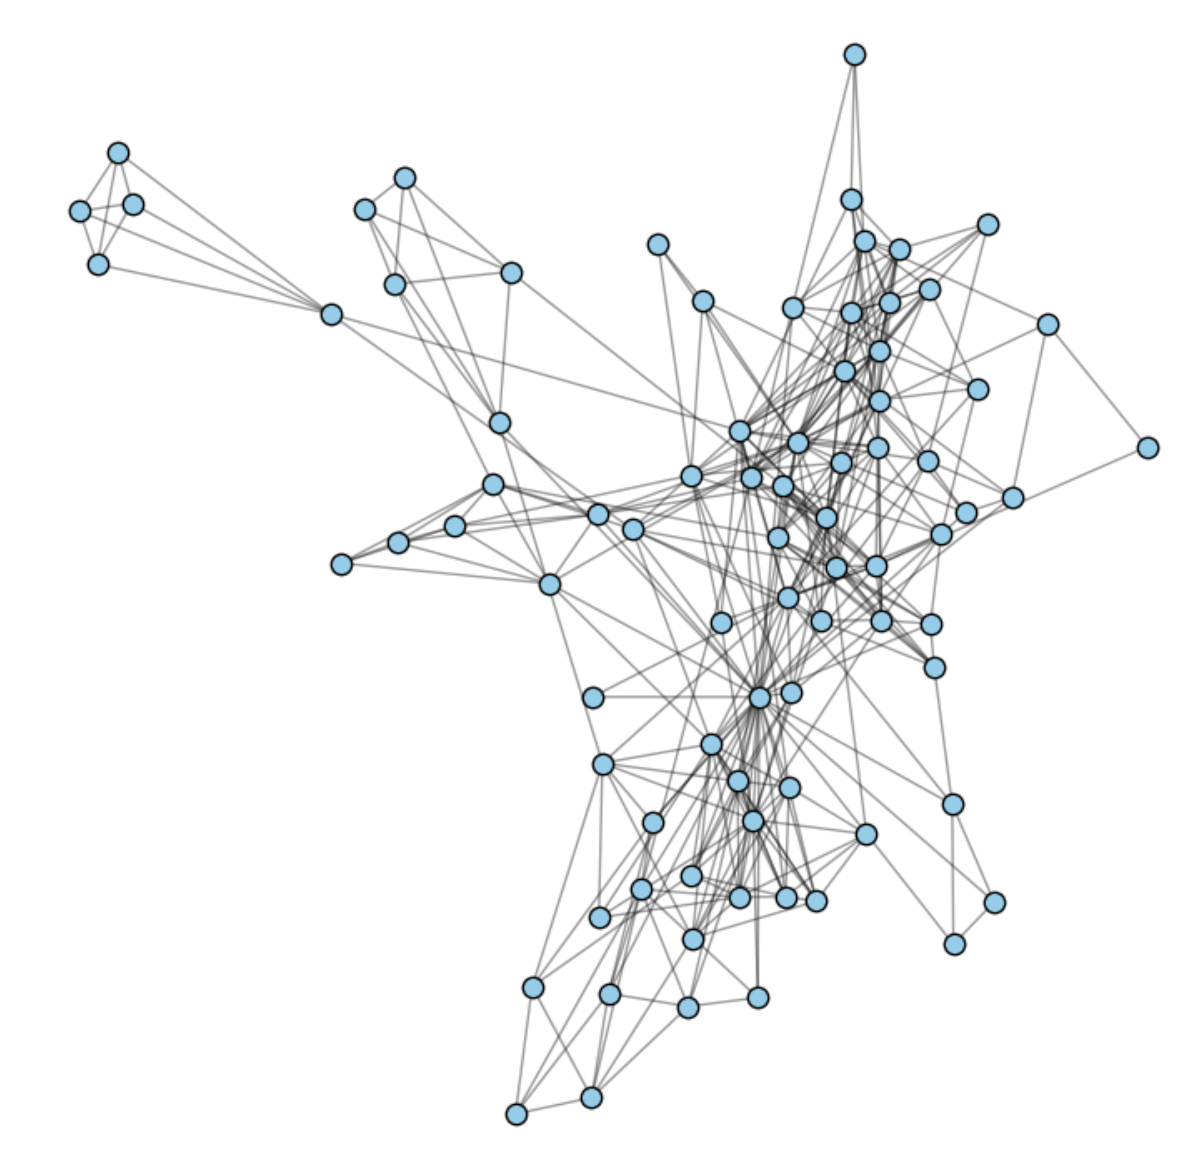
\includegraphics[width=0.75\linewidth]{images/malawi_network.png}
\caption{Réseau de contacts du Malawi}
\end{figure}

% =============================================================
\subsection{Communautés via l'algorithme de Louvain }

Nous obtenons :

\begin{itemize}
    \item \textbf{non pondéré :} 7 communautés, modularité = 0.503 ;
    \item \textbf{pondéré :} 21 communautés, modularité = 0.892.
\end{itemize}

\begin{figure}[H]
\centering
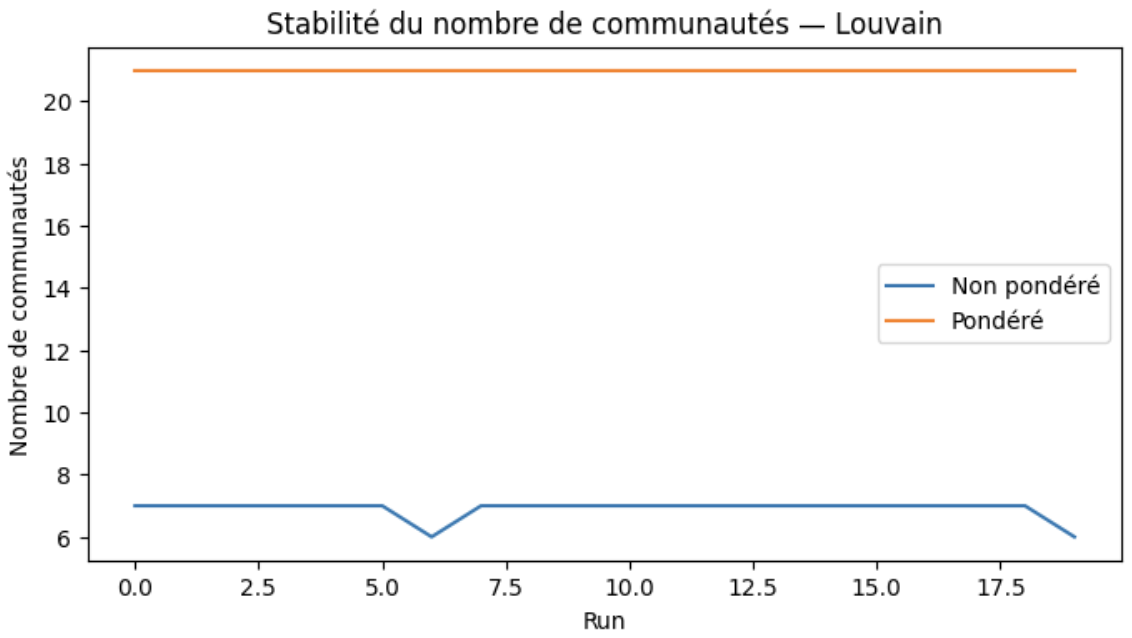
\includegraphics[width=0.70\linewidth]{images/stability_louvain.png}
\caption{Stabilité du nombre de communautés détectées par Louvain}
\end{figure}

\noindent
\textbf{Comparaison avec l’article :}

\begin{itemize}
    \item article : 8 communautés (non pondéré), 13 (pondéré) ;
    \item article : modularité = 0.48 (non), 0.75 (pondéré).
\end{itemize}

Les valeurs non pondérées sont proches de celles de l'article.
En revanche, la modularité pondérée obtenue ici est très élevée
(\textbf{0.89}), indiquant une segmentation plus forte,
due au retrait d’individus faiblement connectés.

% =============================================================
\subsection{Stabilité du Louvain}

Sur 20 exécutions :

\begin{itemize}
    \item non pondéré : oscille entre 6 et 7 communautés ;
    \item pondéré : parfaitement stable à 21 communautés.
\end{itemize}

La stabilité renforcée en pondéré suggère que les poids accentuent
les frontières communautaires (ménages).

% =============================================================
\subsection{Spectre du Laplacien et dynamique de consensus}

Elle permet de caractériser la structure interne du réseau, la présence de communautés
cohésives et la vitesse de diffusion d’une information au sein de la population.

Le Laplacien non pondéré est défini par $L = D - A$, où $A$ est la matrice
d’adjacence et $D$ la matrice des degrés.

\subsubsection*{Valeurs propres du Laplacien}

Le calcul des dix plus petites valeurs propres du Laplacien normalisé du réseau Malawi donne :

\[
\lambda =
\begin{pmatrix}
0 \\
0.0675 \\
0.1334 \\
0.1485 \\
0.2332 \\
0.3044 \\
0.3260 \\
0.3888 \\
0.4706 \\
0.5271
\end{pmatrix}
\]

Ces valeurs appellent plusieurs observations essentielles :

\begin{enumerate}
    \item \textbf{La première valeur propre est  égale à zéro}.  
    Selon le théorème spectral du Laplacien (Chapitre 6 du cours), la multiplicité de la valeur propre nulle correspond au nombre de composantes connexes du réseau.  
    Ici, la multiplicité est égale à 1, ce qui implique que le réseau Malawi nettoyé est entièrement connexe.

    \item \textbf{Différence avec l’article}.  
    L’étude originale rapporte deux composantes connexes (86 nœuds et 355 arêtes).  
    Après nettoyage (suppression des individus très peu actifs), nous obtenons un réseau plus restreint (81 nœuds) mais dans lequel les composantes isolées ont disparu.  
    Cela justifie la présence d’une seule valeur propre nulle.

    \item \textbf{Présence de valeurs propres proches de zéro}.  
    Les valeurs suivantes ($0.0675$, $0.1334$, $0.1485$, etc.) sont petites mais strictement positives.  
    Ces petites valeurs indiquent la présence de \textbf{communautés fortement cohésives}, ce qui est conforme aux observations structurelles du réseau :

    \begin{itemize}
        \item les ménages forment des sous-graphes denses,  
        \item les liens entre ménages sont faibles,
        \item d’où une \textbf{forte modularité} également observée par Louvain et Walktrap.
    \end{itemize}

    \item \textbf{Interprétation dynamique (Consensus)}.  
    Dans la dynamique de consensus $\dot{x} = -Lx$, les petites valeurs propres déterminent les \textbf{temps de mélange} :

    \begin{itemize}
        \item convergence rapide \textit{à l’intérieur des ménages} (forte cohésion structurale),
        \item convergence lente \textit{entre ménages} (faibles connexions inter-households).
    \end{itemize}

    Cette séparation d’échelles temporelles est visible dans nos simulations de consensus
    et correspond parfaitement à l’organisation sociale décrite dans l’article.
\end{enumerate}



\subsubsection*{Interprétation dynamique : convergence du consensus}

La dynamique de consensus étudiée au Chapitre~6 s’écrit :
\[
\dot{x} = -Lx.
\]

Le taux de convergence vers un consensus global dépend fortement de $\lambda_2$,
appelée \textit{Fiedler value}. Dans le réseau Malawi, la valeur très faible de
$\lambda_2 = 0.0674$ implique :

\begin{itemize}
    \item une \textbf{convergence très lente} entre les différentes zones du village ;
    \item mais une \textbf{convergence très rapide à l’intérieur d’un ménage},
          dont les liens internes sont denses.
\end{itemize}

Ce comportement illustre une \textbf{séparation d’échelles temporelles} :

\begin{itemize}
    \item à petite échelle, les individus d’un même foyer harmonisent rapidement leurs comportements
          (interactions fréquentes et régulières) ;
    \item à grande échelle, la diffusion d’information d’un ménage à un autre est plus lente,
          en raison du faible nombre de liens inter-ménages.
\end{itemize}

\subsubsection*{Visualisation de la dynamique}

La Figure~\ref{fig:consensus} illustre une simulation numérique de la dynamique
$\dot{x}=-Lx$, où les valeurs initiales sont distribuées aléatoirement.

\begin{figure}[H]
\centering
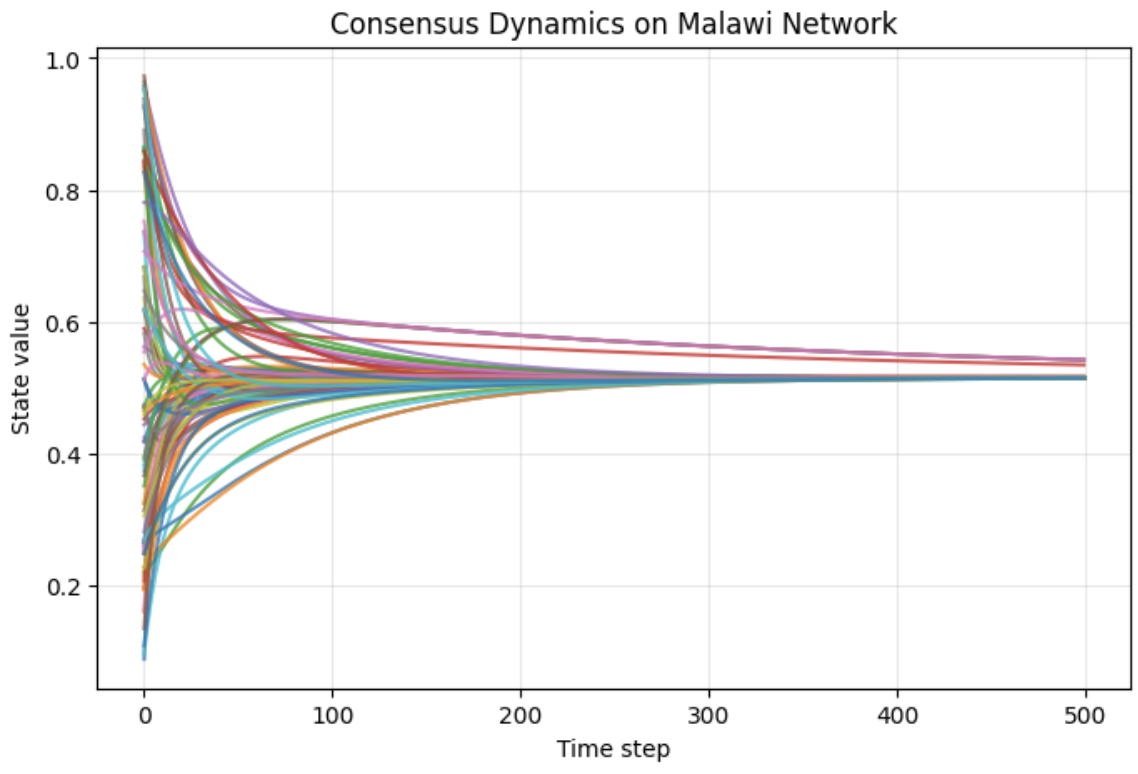
\includegraphics[width=0.85\linewidth]{images/consensus_dynamics.png}
\caption{Dynamique de consensus sur le réseau Malawi. Les ménages convergent rapidement,
alors que le consensus global s'établit lentement.}
\label{fig:consensus}
\end{figure}

On observe clairement une stabilisation rapide à l’intérieur des communautés locales,
suivie d’une phase lente correspondant à la synchronisation inter-ménages.

\subsubsection*{Conclusion sur l'analyse spectrale}

L’étude du spectre du Laplacien fournit une validation mathématique indépendante
de la structure communautaire observée dans l’article.  
Elle démontre que :

\begin{itemize}
    \item les ménages forment des modules cohésifs ;
    \item les interactions inter-ménages sont faibles ;
    \item la diffusion sociale (information, comportements, infections) est fortement contrainte
          par la géographie sociale du village.
\end{itemize}

Ainsi, l'analyse spectrale du réseau confirme pleinement les conclusions sociales et
épidémiologiques de l'étude Malawi.

\subsection{Walktrap }

Walktrap détecte \textbf{8 communautés} avec des tailles variées :
\[
[18,\, 3,\, 24,\, 12,\, 6,\, 5,\, 8,\, 5].
\]



Méthode plus conservative que Louvain pondéré, elle regroupe 
plusieurs ménages proches en une même communauté,
ce qui correspond bien à la structure sociale du village.

% =============================================================
\subsection{Infomap / Flow-based clustering}

Infomap trouve \textbf{7 communautés}.  
Cela correspond presque exactement au Louvain non pondéré,
ce qui indique une structure robuste de “zones de vie”
au sein du village.



% =============================================================
\subsection{Spectral clustering }

En fixant $k = 7$ (comme Louvain non pondéré),  
Spectral clustering produit des communautés plus équilibrées, adaptées
à la structure globale du graphe mais moins sensibles aux ménages.


% =============================================================
\subsection{Analyse multi-échelle : $\gamma$-modularity }

Nous évaluons la partition en fonction du paramètre de résolution $\gamma$ :

\begin{figure}[H]
\centering
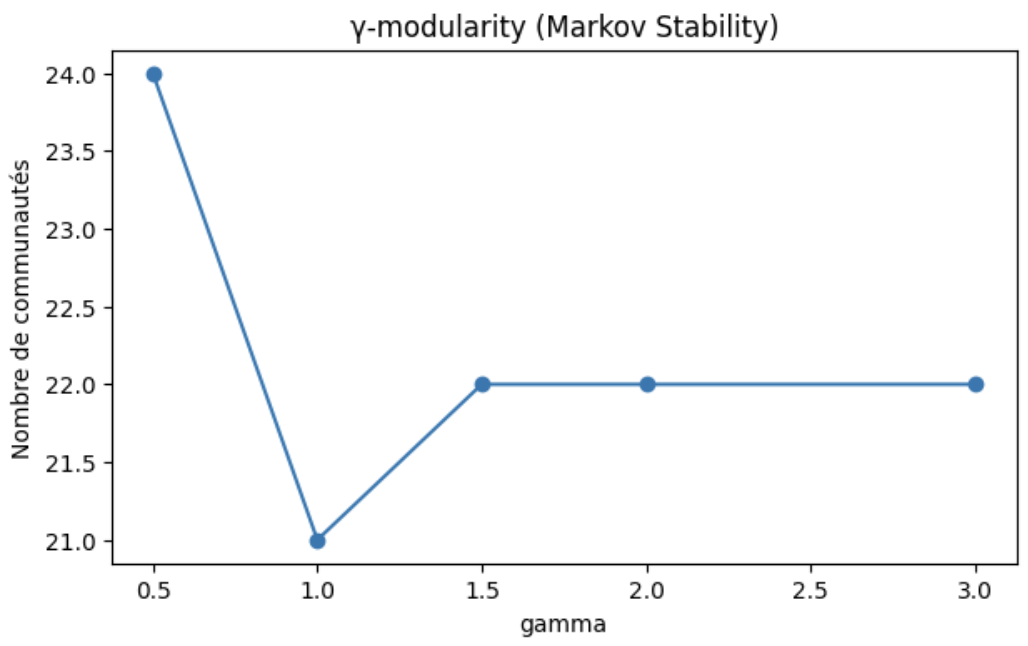
\includegraphics[width=0.70\linewidth]{images/y_modularity.png}
\caption{$\gamma$-modularity : stabilité du nombre de communautés}
\end{figure}

Résultats :

\begin{itemize}
    \item stabilité remarquable pour $\gamma \in [1,3]$ : environ 21–22 communautés ;
    \item montée à 24 communautés pour $\gamma = 0.5$.
\end{itemize}

Cette stabilité révèle une structure multi-échelle robuste, typique des 
réseaux communautaires fortement modulaires comme les ménages malawites.

% =============================================================
\subsection{k-core decomposition}

Le noyau structurel est donné par :

\begin{itemize}
    \item \textbf{k-core maximal = 7} ;
    \item \textbf{31 individus} dans le noyau ;
    \item aucune périphérie (après nettoyage).
\end{itemize}

Ce noyau correspond aux adultes les plus connectés,
adolescents sociables et HSA mentionnés dans l’article.

% =============================================================
\section{Dynamique épidémique}

\subsection{Seuil épidémique}

La plus grande valeur propre du graphe vaut :
\[
\lambda_{\max} = 11.93,
\qquad 
\frac{\beta}{\mu} > \frac{1}{\lambda_{\max}} = 0.0838.
\]

Cela signifie qu’une infection même modérément contagieuse
(\(\beta > 0.08 \mu\)) peut se propager dans toute la population.

% -------------------------------------------------------------
\subsection{Identification des superspreaders}

Les individus les plus centraux selon la distribution stationnaire du random walk sont :

\[
16,\; 81,\; 69,\; 74,\; 70.
\]

Ils possèdent simultanément un fort degré, une forte eigenvector centrality
et une centralité de flux élevée : ce sont clairement les “super-contacteurs”
du village.

% -------------------------------------------------------------
\subsection{Simulation SIR}

\begin{figure}[H]
\centering
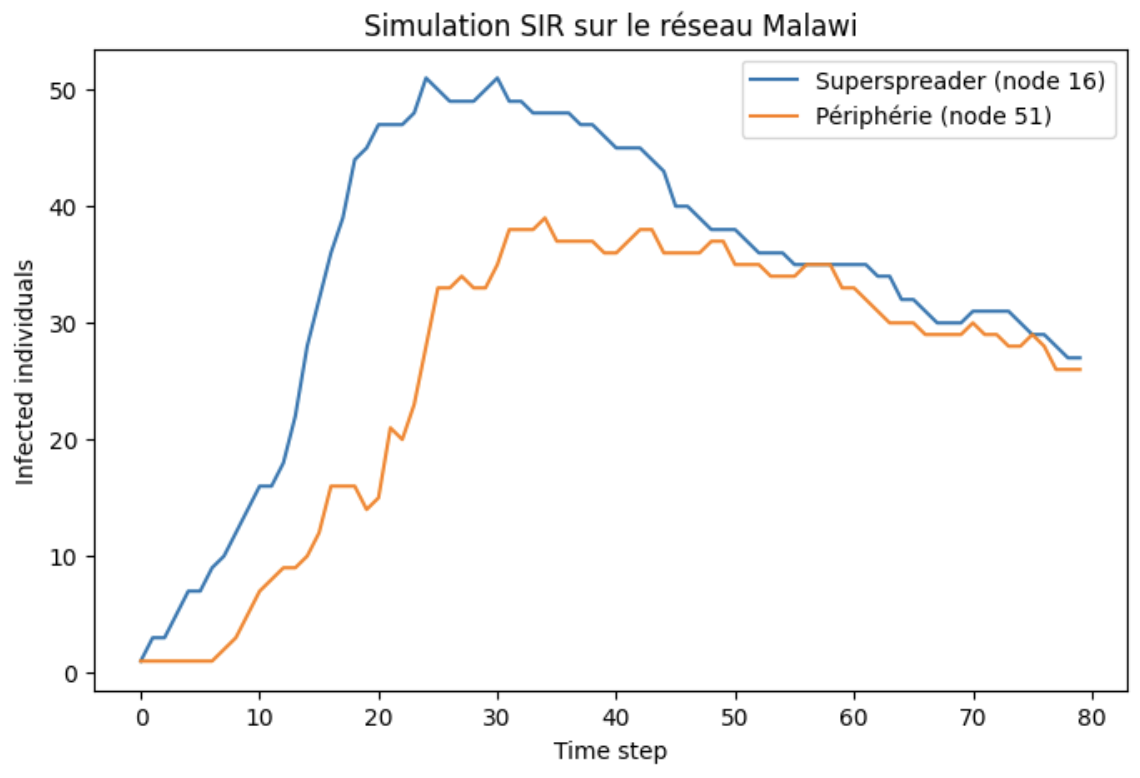
\includegraphics[width=0.75\linewidth]{images/sir.png}
\caption{Simulation SIR : superspreader vs individu périphérique}
\end{figure}

\begin{itemize}
    \item Patient zéro = superspreader : épidémie massive ($>50$ infectés).
    \item Patient zéro = périphérie : propagation presque nulle.
\end{itemize}

Ce résultat confirme empiriquement les conclusions de l’étude Malawi :
la structure du réseau influence fortement la dynamique épidémique.


\end{document}


